\documentclass[pscyr, 12pt]{hedlab}
\usepackage[russian]{babel}
\usepackage{graphicx}

\graphicspath{{images/}}

\labname{Разработка баз данных в СУБД Oracle}
\labnum{6}
\student{Голубев~А.~В., САПР-1.1п}
\labdate{}

\begin{document}
    \makeheader
    \noindent\textbf{Цель:} создание табличного отчёта

    \noindent\textbf{Постановка задачи:}
    \vspace*{-1em}
    \begin{itemize}\itemsep-5pt
        \item изучить функциональные возможности программы
        \item создать табличный отчёт 
        \item вывести данные на экран
    \end{itemize}

    Используем мастер \emph{Block Wizard} для создания отчёта
    \begin{figure}[ht!]
        \center
        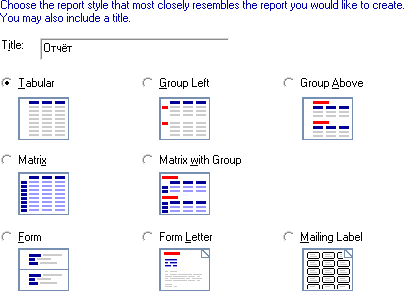
\includegraphics[width=0.47\textwidth]{lab06_01}
    \end{figure}

    Выбираем тип запроса
    \begin{figure}[ht!]
        \center
        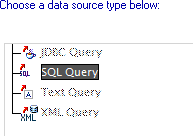
\includegraphics[width=0.47\textwidth]{lab06_02}
    \end{figure}

    \pagebreak

    Определяем выводимые поля
    \begin{figure}[ht!]
        \center
        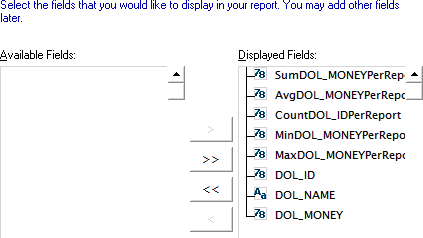
\includegraphics[width=0.47\textwidth]{lab06_03}
    \end{figure}

    Определяем подсчитываемые поля
    \begin{figure}[ht!]
        \center
        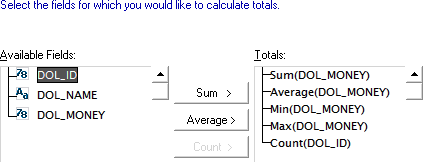
\includegraphics[width=0.47\textwidth]{lab06_04}
    \end{figure}

    Редактируем \emph{label}-метки полей
    \begin{figure}[ht!]
        \center
        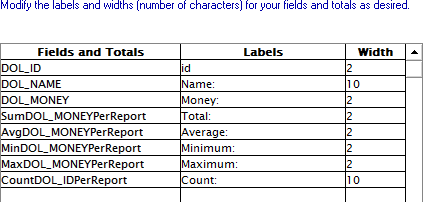
\includegraphics[width=0.47\textwidth]{lab06_05}
    \end{figure}

    Выбираем шаблон отсчёта
    \begin{figure}[ht!]
        \center
        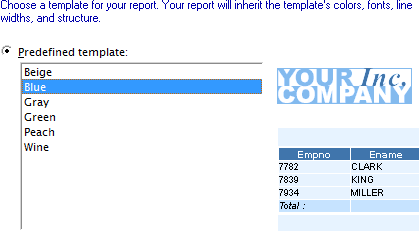
\includegraphics[width=0.47\textwidth]{lab06_06}
    \end{figure}

    \pagebreak

    Структура SQL-запроса
    \begin{figure}[ht!]
        \center
        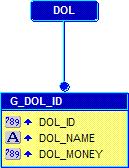
\includegraphics[width=0.2\textwidth]{lab06_08}
    \end{figure}

    Результат выполнения
    \begin{figure}[ht!]
        \center
        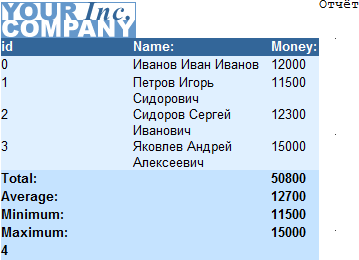
\includegraphics[width=0.47\textwidth]{lab06_07}
    \end{figure}

    \noindent\textbf{Вывод:} в результате проделанной работы
    \vspace*{-1em}
    \begin{enumerate}\itemsep-5pt
        \item создан отчёт по таблице из БД
        \item использованы команды для расчёта дополнительных полей
        \item изучен базовый функционал программы формирования отчётов
    \end{enumerate}
\end{document}